%presentation declaration
\documentclass[10pt]{beamer}
\usetheme{metropolis}

%packages
%beamer stuff
\usepackage{appendixnumberbeamer}
\usepackage{booktabs}
\usepackage[scale=2]{ccicons}
\usepackage{pgfplots}
\usepgfplotslibrary{dateplot}
\usepackage{xspace}
%language
\usepackage[brazilian]{babel}
\usepackage[utf8]{inputenc}
%images
\usepackage{graphicx}
\usepackage{float}

%macros
\newcommand{\tit}[1]{\textit{#1}}
\newcommand{\tbf}[1]{\textbf{#1}}
\newcommand{\ttt}[1]{\texttt{#1}}

%title
\title{Atenção Visual Eficiente com Deep Learning}
\subtitle{}
\author{Erik Perillo, Esther Colombini}
\date{}
\institute{Instituto de Computação -- Unicamp}

\begin{document}

\maketitle

\section{Introdução}

\begin{frame}{}
    \begin{figure}
        \centering
        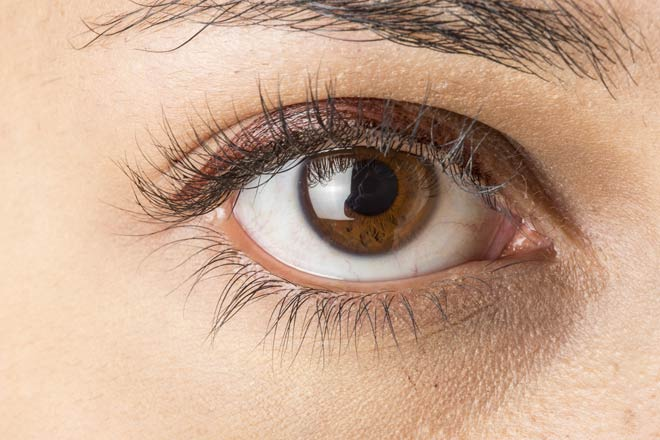
\includegraphics[width=1.0\linewidth]{./img/eye.jpg}
    \end{figure}
\end{frame}

\begin{frame}{}
    \begin{figure}
        \centering
        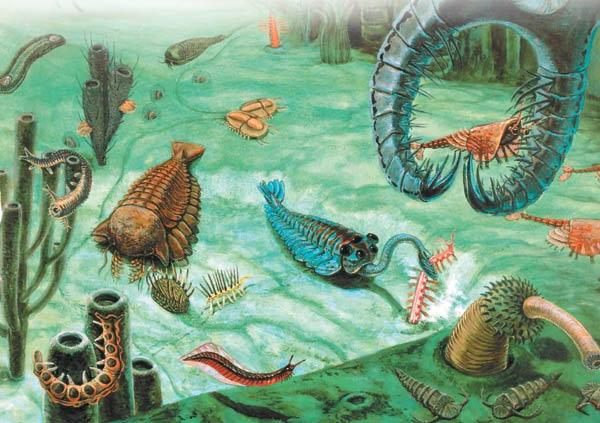
\includegraphics[width=1.0\linewidth]{./img/precambrian}
    \end{figure}
\end{frame}

\begin{frame}{}
    \begin{figure}
        \centering
        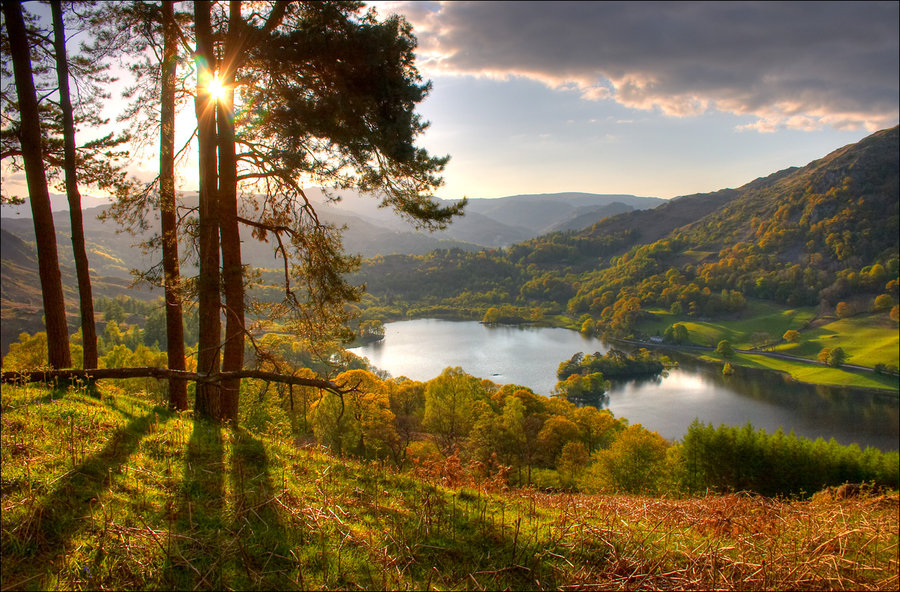
\includegraphics[width=1.0\linewidth]{./img/beautiful_landscape.jpg}
    \end{figure}
\end{frame}

\begin{frame}{}
    \begin{figure}
        \centering
        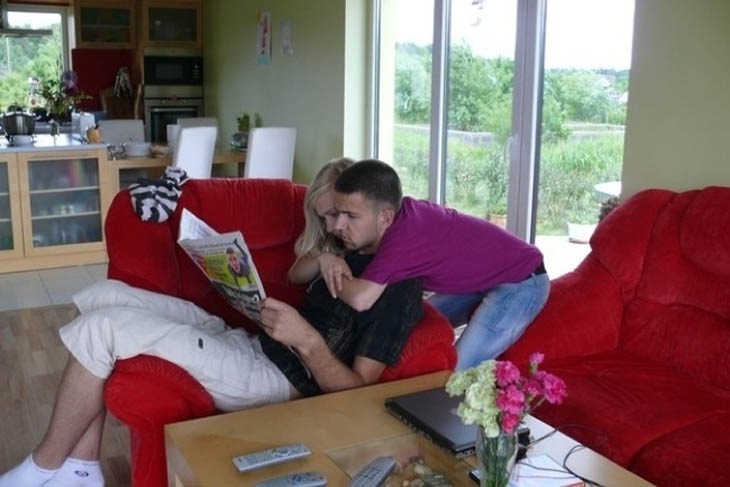
\includegraphics[width=1.0\linewidth]{./img/confusing_image_4.jpg}
    \end{figure}
\end{frame}

\begin{frame}{}
    \begin{figure}
        \centering
        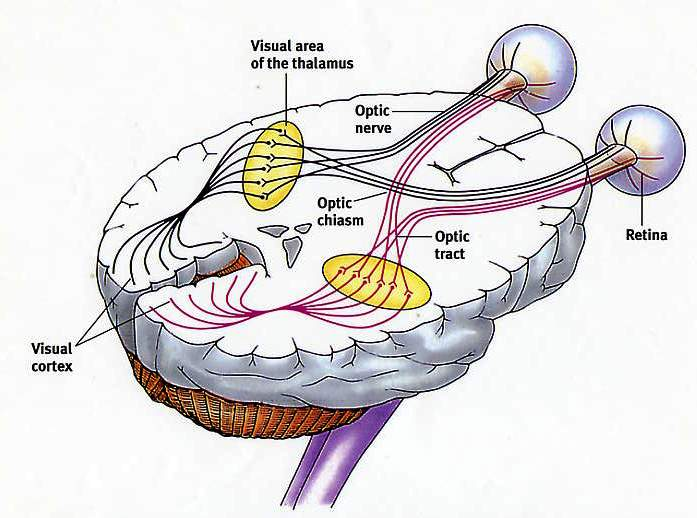
\includegraphics[width=0.9\linewidth]{./img/visual_system_brain.jpg}
    \end{figure}
\end{frame}

\begin{frame}{}
    \begin{figure}
        \centering
        
\includegraphics[width=0.9\linewidth]{./img/wheres_wally.jpg}
    \end{figure}
\end{frame}

\begin{frame}{}
    \begin{figure}
        \centering
        
\includegraphics[width=0.9\linewidth]{./img/wheres_wally_focus_1.jpg}
    \end{figure}
\end{frame}

\begin{frame}{}
    \begin{figure}
        \centering
        
\includegraphics[width=0.9\linewidth]{./img/wheres_wally_focus_2.jpg}
    \end{figure}
\end{frame}

\begin{frame}{Atenção Visual}
    \begin{quote}
        Seleção de uma certa região espacial do campo visual para
        posterior processamento cognitivo
    \end{quote}
\end{frame}

\begin{frame}{Atenção: Top-down versus Bottom-up}
    \begin{itemize}[<+->]
        \item Top-down: Estímulo interno do ser que direciona a atenção
            a padrões específicos de estímulo visual
        \item \tbf{Bottom-up (saliência visual):}
            Estímulo externo que capta a atenção visual
    \end{itemize}
\end{frame}

\begin{frame}{}
    \begin{figure}
        \centering
        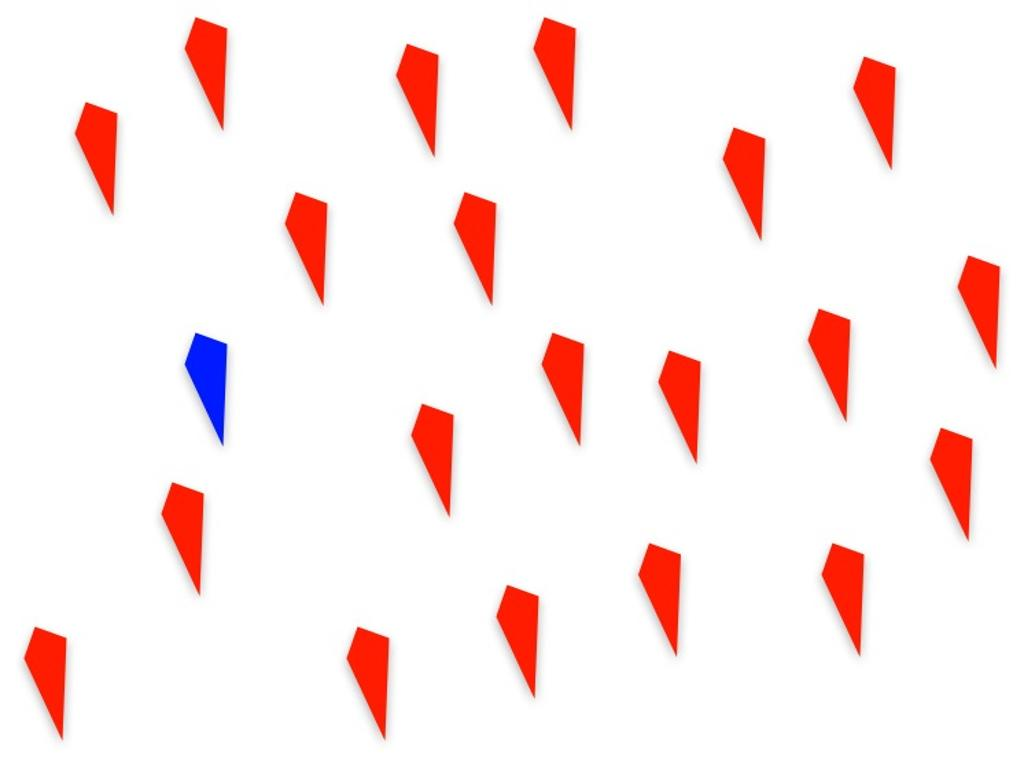
\includegraphics[width=0.8\linewidth]{./img/syntheticData2.jpg}
    \end{figure}
\end{frame}

\begin{frame}{}
    \begin{figure}
        \centering
        
\includegraphics[width=0.8\linewidth]{./img/syntheticData5.jpg}
    \end{figure}
\end{frame}

\begin{frame}{}
    \begin{figure}
        \centering
        
\includegraphics[width=0.8\linewidth]{./img/syntheticData1.jpg}
    \end{figure}
\end{frame}

\begin{frame}{}
    \begin{figure}
        \centering
        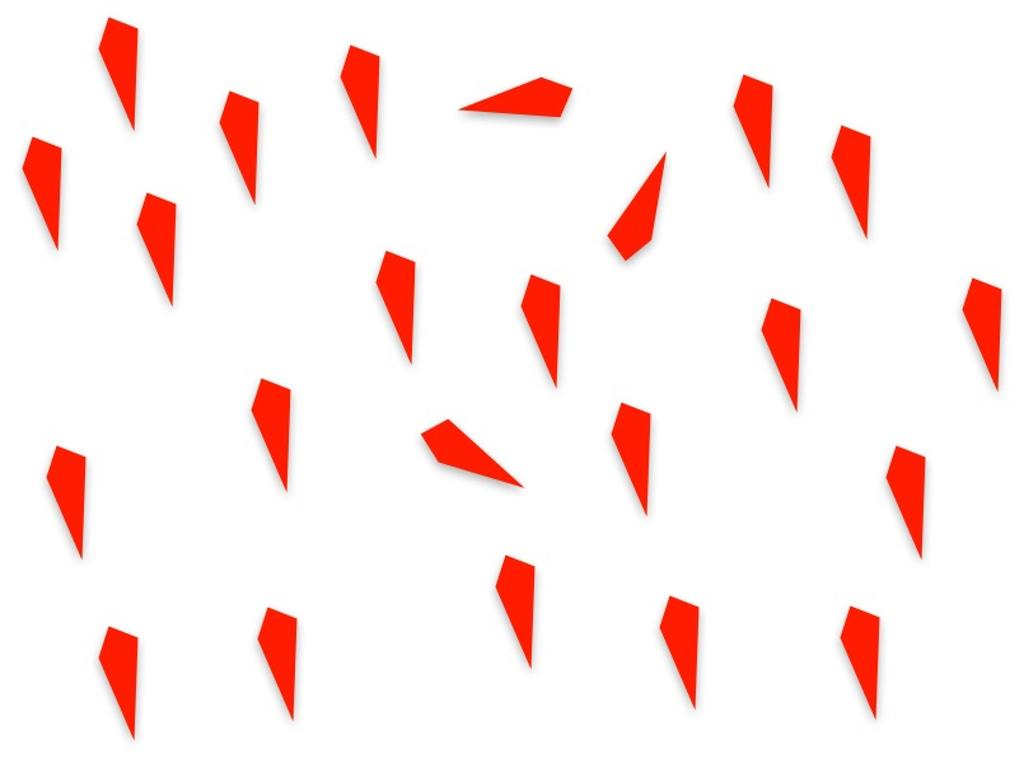
\includegraphics[width=0.8\linewidth]{./img/syntheticData3.jpg}
    \end{figure}
\end{frame}

\begin{frame}{}
    \begin{figure}
        \centering
        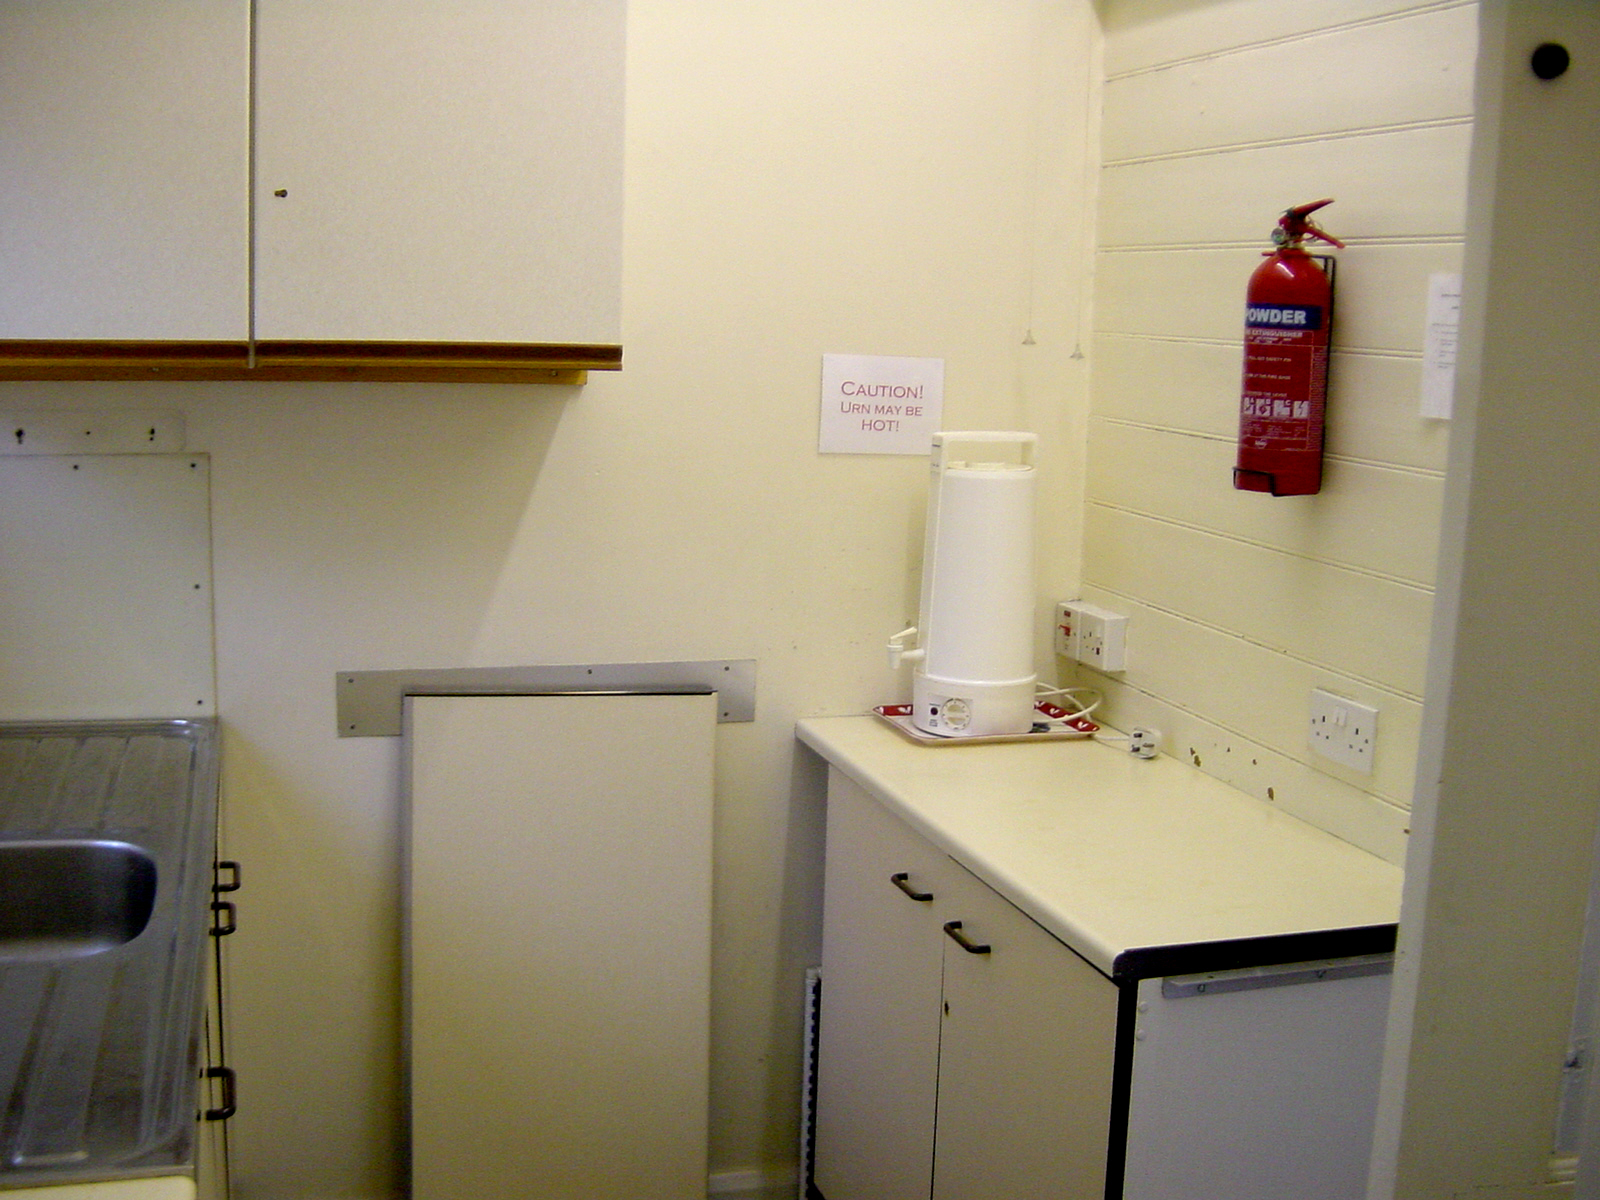
\includegraphics[width=0.9\linewidth]{./img/fire_extinguisher.jpg}
    \end{figure}
\end{frame}

\begin{frame}{Mapa de saliência}
    \begin{figure}
        \centering
        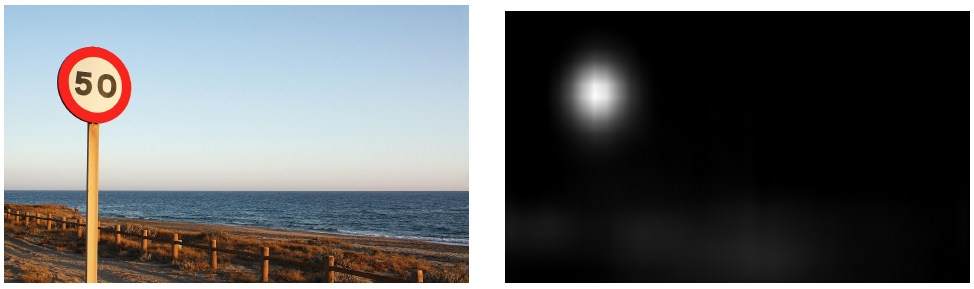
\includegraphics[width=1.0\linewidth]{./img/saliency_map_ex_1.png}
    \end{figure}
\end{frame}

\begin{frame}{}
    \begin{center}
        \begin{tabular} {cc}
        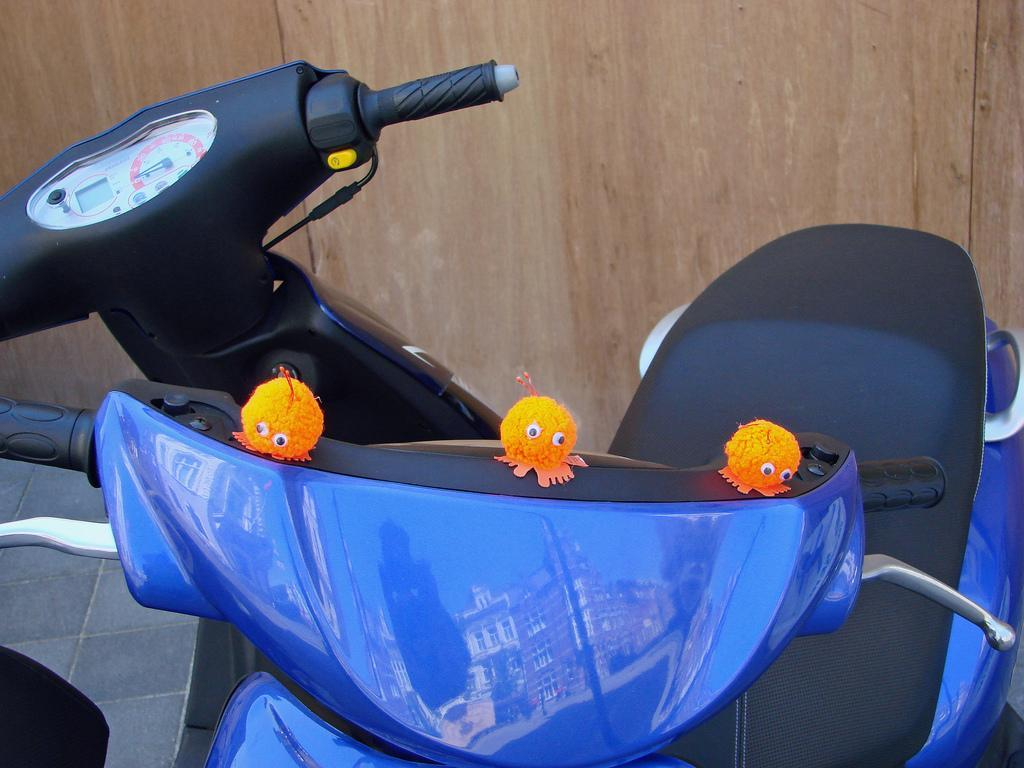
\includegraphics[width=0.45\textwidth]{./img/orange_balls.jpg} &
        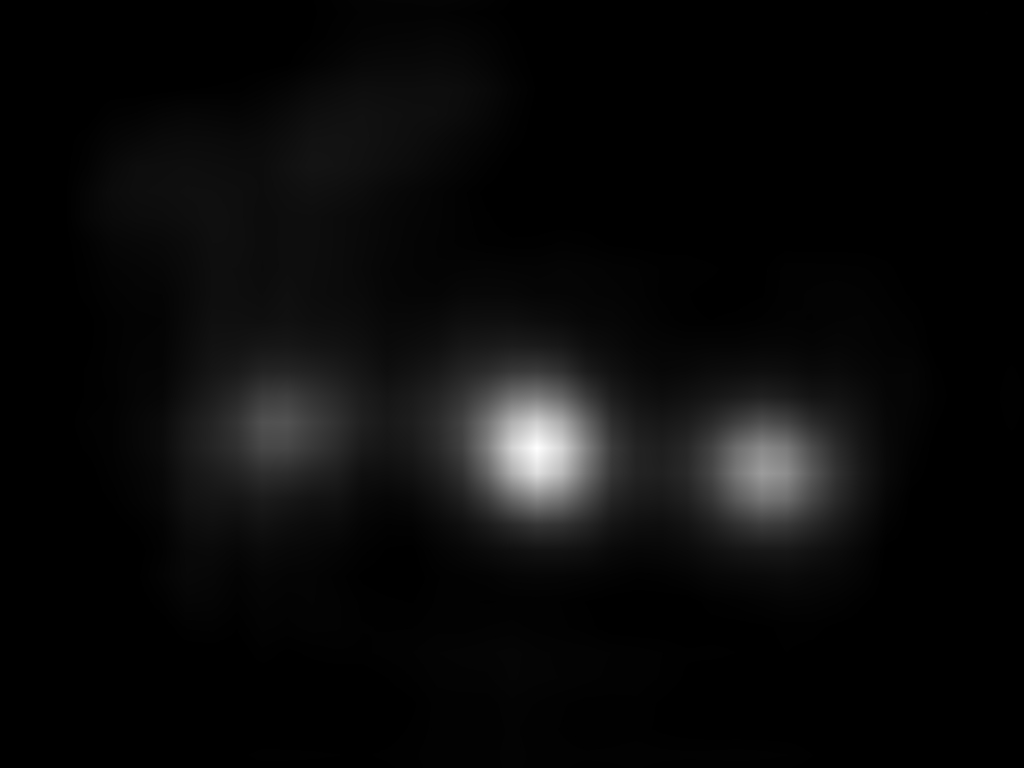
\includegraphics[width=0.45\textwidth]{./img/orange_balls_map.jpg}
        \end{tabular}
    \end{center}
\end{frame}

\begin{frame}{}
    \begin{center}
        \begin{tabular} {cc}
        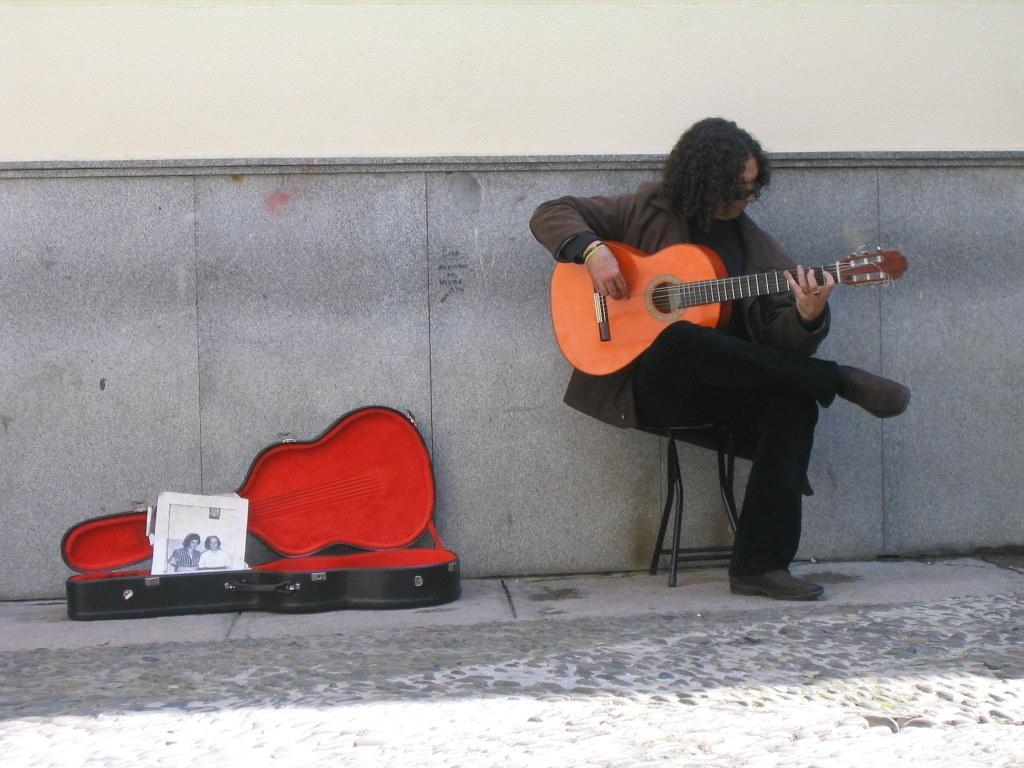
\includegraphics[width=0.45\textwidth]{./img/guitarist.jpg} &
        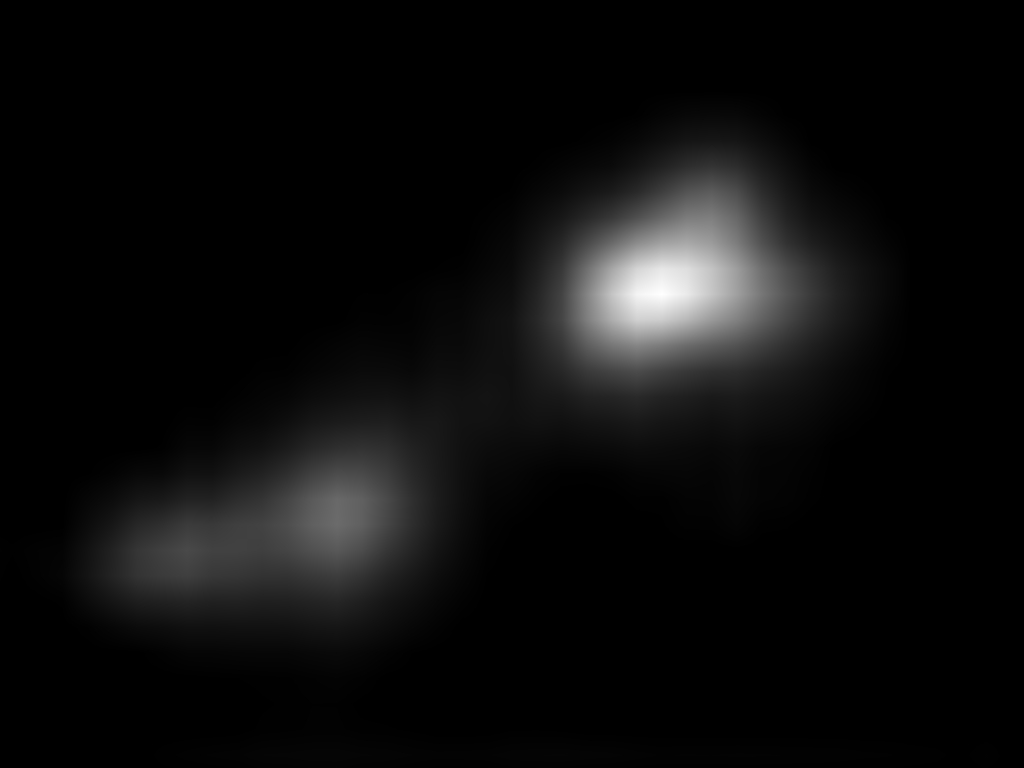
\includegraphics[width=0.45\textwidth]{./img/guitarist_map.jpg}
        \end{tabular}
    \end{center}
\end{frame}

\begin{frame}{}
    \begin{center}
        \begin{tabular} {cc}
        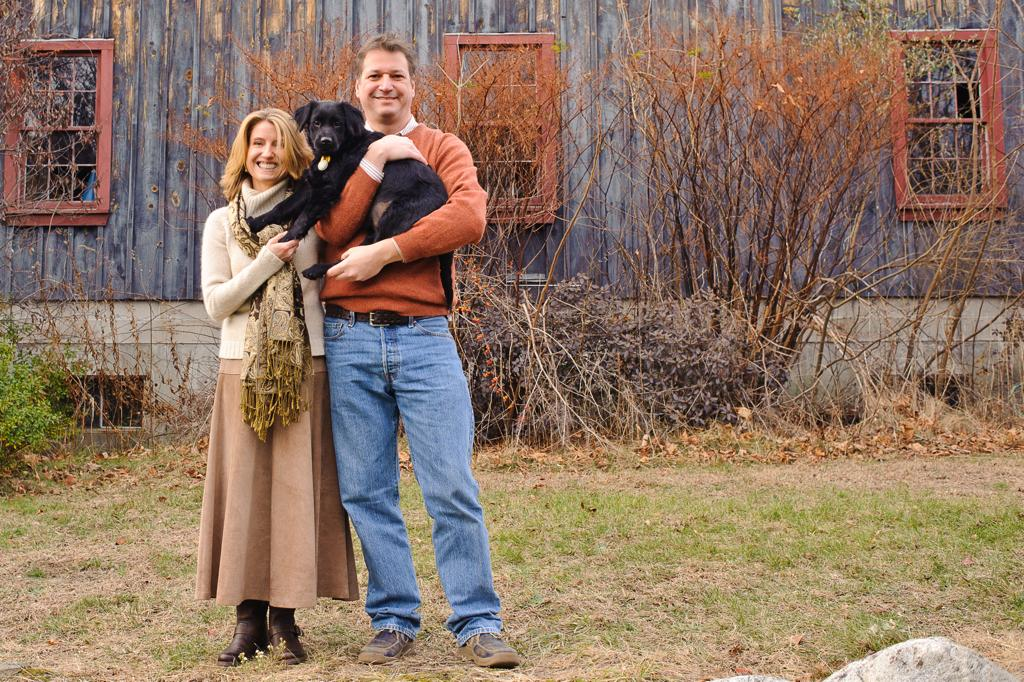
\includegraphics[width=0.45\textwidth]{./img/couple.jpg} &
        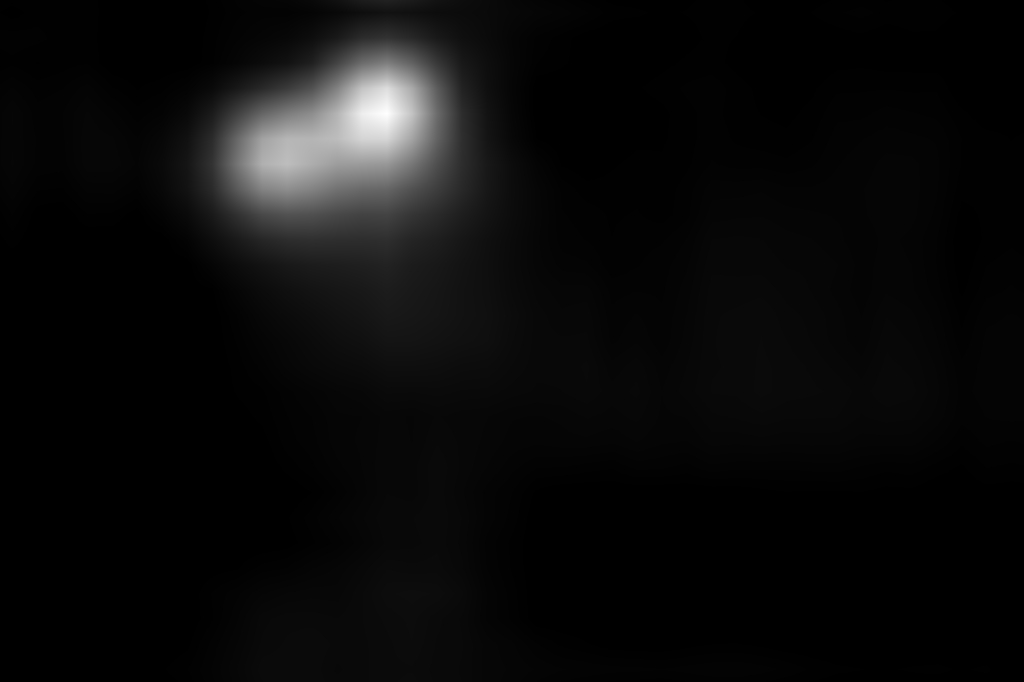
\includegraphics[width=0.45\textwidth]{./img/couple_map.jpg}
        \end{tabular}
    \end{center}
\end{frame}

\begin{frame}{}
    \begin{quote}
        Podemos fazer um computador identificar saliências visuais?
    \end{quote}
\end{frame}

\begin{frame}{Modelo de saliência visual}
    \tbf{Ideia:}
    \begin{itemize}[<+->]
        \item Dada uma imagem, gerar um mapa de saliência coerente
            com o que humanos gerariam
    \end{itemize}
\end{frame}

\begin{frame}{Modelo de saliência visual}
    \tbf{Problemas:}
    \begin{itemize}[<+->]
        \item Saliência emerge de relações muito complexas em imagens normais
        \item É difícil captar todas as nuances envolvidas apenas extraindo
            \tit{features} pré-determinadas
    \end{itemize}
\end{frame}

\begin{frame}{}
    \begin{center}
        \begin{tabular} {cc}
        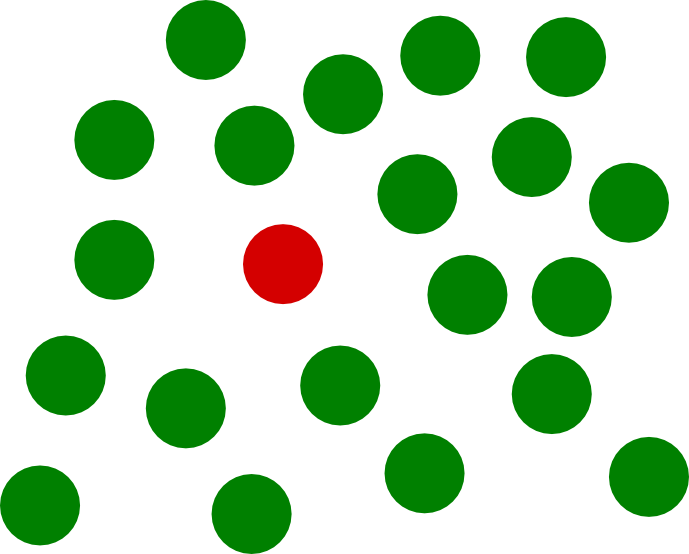
\includegraphics[width=0.45\textwidth]{./img/red_in_green.png} &
        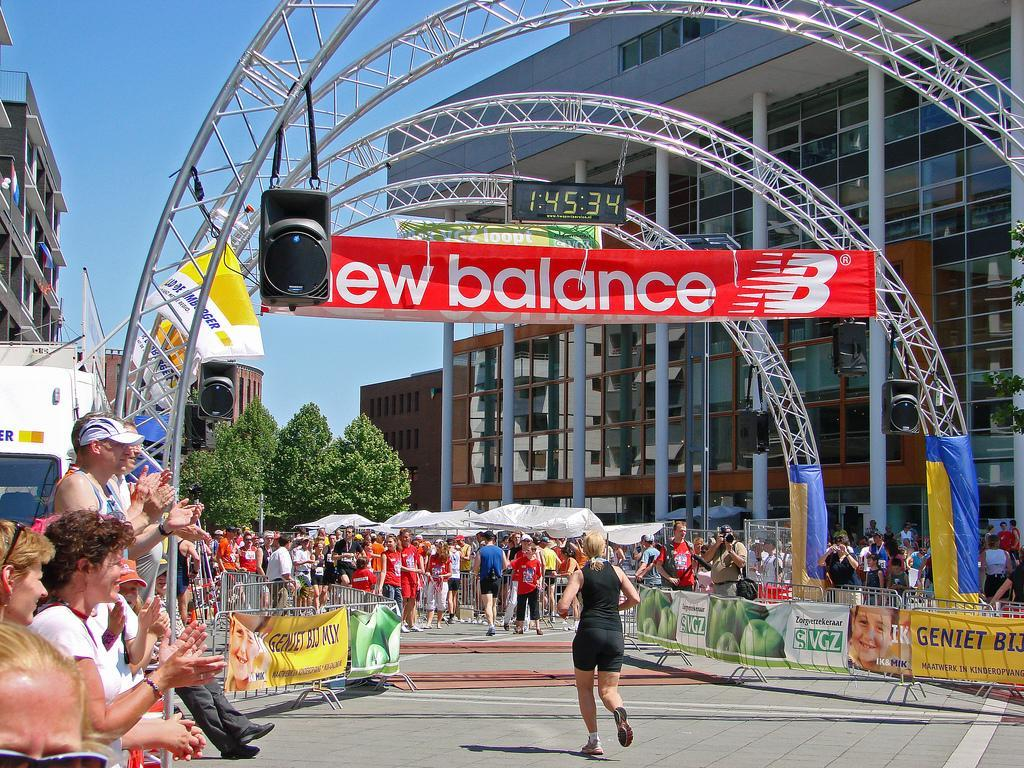
\includegraphics[width=0.45\textwidth]{./img/running_people.jpg}
        \end{tabular}
    \end{center}
\end{frame}

\section{Modelo Proposto}

\begin{frame}{Arquitetura da rede}
\end{frame}

\begin{frame}{Inception}
\end{frame}

\begin{frame}{Pré-processamento}
\end{frame}

\begin{frame}{Treinamento}
\end{frame}

\section{Resultados}

\begin{frame}{Exemplos}
\end{frame}

\begin{frame}{MIT300 Benchmark}
\end{frame}

\begin{frame}{Conclusões}
\end{frame}

\begin{frame}{Referências}
\end{frame}

\end{document}
